\documentclass[a4paper,12pt]{article} % тип документа

\usepackage{tikz}
\usepackage[T2A]{fontenc}			% кодировка
\usepackage[utf8]{inputenc}			% кодировка исходного текста
\usepackage[english,russian]{babel}	% локализация и переносы
\usepackage{amsfonts,longtable}

% Математика
\usepackage{amsmath,amsfonts,amssymb,amsthm,mathtools} 


\usepackage{wasysym}

\title{Лабораторный журнал 1.4.5 по курсу \\ "Общая физика"  \\ 
\vspace{0.2cm}
\vspace{4.5cm}
 \LARGE{\textbf{Изучение колебаний струны}}\vspace{5.5cm}}
\date{26.10.2018}
\usepackage{tikz}
\author{\vspace{0.2cm}Баринов Леонид}

\begin{document}
\maketitle
\newpage
\section{Цель работы} Изучение поперечных стоячих волн на струне; определение собвственных частот колебаний струны; исследование зависимости скорости распространения поперечных волн на струне в зависимости от её натяжения.

\section{Теоритические данные}
\subsection{Введение}
Второй закон Ньютона для вертикального движения элемента струны:
\begin{equation}
\delta m \frac{\partial^2 y}{\partial t^2} = -T_1\sin\alpha_1 + T_2\sin\alpha_2
\end{equation}
$T_1$ и $T_2$ - силы натяжения, действующие на элемент струны, возникающие при отклонении от равновесия и направленные по касатлеьной к струне

Скорость распространения волн на струне:
\begin{equation}
u = \sqrt{\frac{T}{\rho_l}}
\end{equation}

Уравнение свободных малых поперечных колебаний струны: 
\begin{equation}
\frac{\partial^2 y}{\partial t^2} = u^2\frac{\partial^2 y}{\partial x^2}
\end{equation}
Уравнение (3) называют волновым уравнением. Кроме волн на струне, оно может описывать волновые процессы в самых разных системах, в том числе волны в сплошных средах(звук), электромагнитные волны и т. д.
\subsection{Бегущие волны}
Решение диффуренциального уравнения в частных производных (3) предмтавимо в виде суммы двух волн произвольной формы, бегущих в противоположные стороны со скоростями $\pm u$:
\begin{equation}
y(x, t) = y_1(x-ut)+y_2(x+ut),
\end{equation}
где $u$ -- скорость распространения волны (2), $y_1$ и $y_2$ -- проивзольные функции, вид которых в конкретной задаче определяется из начальных и граничных условий.

Особый интерес представляет случай гармонических волн:
\begin{equation}
y(x, t) = a\cos[k(x-ut)] + b\cos[k(x+ut)] = a\cos(\omega t-kx)+b\cos(wt+kx)
\end{equation}

Выражение (5) представляет собой супрепозицию двух гармонических волн, бегущих навстречу друг другу со скоростью
\begin{equation}
u = \frac{\omega}{k}=\nu\lambda
\end{equation}
Их \textit{длина волны} $\lambda = \frac{2\pi}{k}$, \textit{частота} $\nu = \frac{\omega}{2\pi}$. Величина $k = \frac{2\pi}{\lambda}$ называется волновым числом или пространственной частотой волны.
Заметим, что формула (2) означает, что скорость $u$ распространения поперечных волн на струне зависит только от силы натяжения струны $T$ и ее погонной плотности $\rho_l$.
\subsection{Собственные колебания струны. Стоячие волны}
Функция, описывающая стоячие волны:
\begin{equation}
y(x, t) = 2a \sin kx\cdot \sin\omega t
\end{equation}
Видно, что стоячая волна может быть получена как сумма (интерференция) двух гармонических бегущих волн, имеющих равную амплитуду и двужущихся навстречу друг другу.

Как видоно из (7), точки струны, в которых $sinkx = 0$, в любой момент времени неподвижны. Такие точки называются узлами. Остальные точки совершают в вертикальной плоскости гармонические колебания с частотой
\[\nu = \frac{\omega}{2\pi}=\frac{u}{\lambda}\]
Амплитуда колебаний распределена вдоль струны по гармоническому закону: $y_0(x) = 2a\sin kx$. В точках, нде $\sin kx = 1$, амплитуда колебаний максимальна -- они называются пучностями. Между двумя соседними узлами все участки струны колеблются в фазу (их скорости имеют одинаковое направление), а при переходе через узел фаза колебаний меняется на $\pi$ вследствие изменения знакак $\sin kx$.

Исользуя второе граничное условие $y(L, t)=0$ (точки крепления струны должны быть узлами стоячей волны), найдем условие образования стоячих волн на струне: $y(x, t) = 2a\sin kL\cdot \sin \omega t = 0$, откуда
\[\sin kL = 0 \rightarrow kL = n\frac{\pi}{2},  n\in \mathbb{N}\] 
Таким образом, стоячие волны на струне с закрепленными концами могут образовываться только если на длине струны укладыается целое число полуволн:
\begin{equation}
L = \frac{\lambda_n}{2}n
\end{equation}
Поскольку длина волны однозначно связана с ее частотой, струна может колебаться только с определенными частотами:
\begin{equation}
\nu_n = \frac{u}{\lambda_n}=\frac{n}{2L}\sqrt{\frac{T}{\rho_l}}, n\in \mathbb{N}
\end{equation}
Набор (спектр) расзерешенных частот $\nu_n$ называют собственными частотами колебаний струны. Режим колебаний соответсвующий каждой из частот $\nu_n$, называется собственной (или нормальной) модой колебаний. Проивзольное колебание струны может быть представленно в виде суперпозиции ее собственных колебаний. Наименьшая частота $\nu_1$ называется также основным тоном (или первой гармоникой), а остальные ($\nu_2 = 2\nu_1, \nu_3 = 3\nu_1, ...)$ - обертонами (высшими грамониками). Термин "гармоника иногда употребляется в общем смысле -- как элементарная составляющая сложного гармонического колебания.

На Рис. 1 показана картина стоячих волн для $n = 1, 2, 3$. Заметим, что число $n$ определяет число пучностей (но не узлов!) колеблющейся струны.

Таким образом спектр собственных частот струны определен ее погонной плотностью $\rho_l$, силой натяжения $T$ и длиной струны $L$ (отдельно отметим, что собственные частоты не зависят от модуля Юнга материала струны).
\begin{figure}[h]
\centering
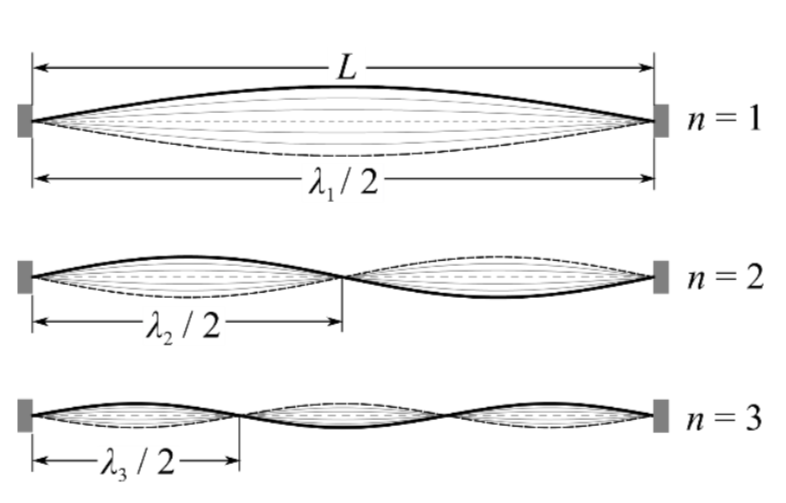
\includegraphics[scale=0.5]{2}
\caption{Стоячие волны (собственные моды колебаний струны) для $n =1, 2, 3$}
\end{figure}
\subsection{Возбуждение колебаний струны}
При колебаниях реальной струны всегда имеет место потеря энергии (часть теряется вследствие трения о воздух, другая часть уходит через неиделаьно закрепленные концы струны и т. д.). Поддержание незатухающих колебаний в струне может осуществляться точенчным источником, в качестве которого в данной работе использует электромагнитный вибратор. При этом возникает необходимость переноса энергии от источника по всей струне.

Рассмотрим вопрос о передаче энергии по струне. В стоячей волне поток энергии вдоль струны отсутствует -- колебательная энергия, заключенная в отрезке струны между двумя соседними узлами, не транспортируется в другие части струны. В каждом таком отрезке проиходит перодическое (дважды за период) превращение кинетической энергии в потенциальную и обратно. Передача энергии между различными участками струны возможно только благодаря бегущим волнам, которые, однако, в рассмотренной выше идеальной модели струны не возникают. Парадокс снимается, если учесть, что из-за потерь энергии при отражении волны от концов не проиходит полной компенсации пдающей и отраженной волны, поэтому к стоячей волне на струне добавляется малая бегущая компонента -- именно она служит "разносчиком" энргии по всей системе. 

Для эффективной раскачки колебаний используется явление резонанса -- вынуждающая частота $\nu$ должна совпадать с одной из собственных частот струны $\nu_n$ (см. (9)). Когда потери энергии в точности компенсируются энергией, поступающей от вибратора, колебания струны становятся стационарными и на ней можно наблюдать стоячие волны. Если потери энергии за период малы по сравнению с запасом колебательной энергии в струне, то искажение стоячих волн бегущей волной не существенно — наложение бегущей волны малой амплитуды на стоячую визуально приводит к незначительному «размытию» узлов. Для достижения максимального эффекта от вибратора, его следует располагать вблизи узловой точки. Это можно показать из следующих элементарных соображений. Пусть вибратор, размещённый в точке $x_0$, способен раскачать соответствующий элемент струны до амплитуды . Если частота вибратора близка к резонансной (т.е. собственной), то как следует из (7), амплитуда колебаний струны в пучности будет равна $2a = \frac{A}{\sin kx_0}$. Таким образом, максимальная раскачка струны достигается, если значение $\sin kx_0$ устремить к нулю, что и соответсвует положениям узлов (из идеализированной модели струны следует, что при размещении вибратора в узле амплитуда колебаний устремится к бесконечности, однако в реальности она ограничивается силами трения и нелинейными эффектами).

Заметим также, что при наблюдении стоячих волн важно, чтобы колебания происходили в одной (вертикальной) плоскости, т. е. были поляризованы. Кроме того, важно, чтобы колебания струны проиходили с малой амплитудой, поскольку при сильном возбуждении нарушаются условия применимости волнового уравнения (3), и в опыте наблюдаются искажения, связанные с нелинейными эффектами.
\section{Экспериментальная установка:}
Схема установки приведена на Рис. 1. Стальная гитарная струна 1 закрепляется в горизонатльной положении между двумя стойками с зажимами 2 и 3, расположенными на массивной станине 4. Один конец струны закреплен в зажиме 2 неподвижно. К противоположному концу струны, перекинутому через блок, прикреплена платформа с грузами 5, создающими натяжение струны. Зажим 3 можно передвигать по станине, устанавливая требуемую длину струны. Возбуждение и регистрация колебаний струны осуществяются с помощью электромагнитных датчиков (вибраторов), расположенных на станине под струной. Электромагнитный датчик 6 подключен к звуковому генератору 7 и служит для возбуждения колебаний струны, частота которых измеряется с помощью частотомера 10 (в некоторых установках частомер встроен в генератор). Колебания струны регитрируются с помощью электромагнитного датчика 8, сигнал которого передается на вход осциллографа 9. Разъемы, через которые датчики с помощью кабелей соединяются с генератором и осциллографом, расположены на корпусе станины.
\subsection{Измерения с помощью осциллографа}
Дли регистрации колебаний струны в работе используется электронный осциллограф, соединенный с электромагнитным датчиком 8. Он позволяет регистрировать колебания в случаях, когда это невозможно сделать визуально. Также с помощью оциллографа можно измерять амплитуду возбуждения и форму сигнала, что дает возможность установить, является ли режим возбуждения стоячих волн линейным, иными словами, имеет ли место прямая пропорциональность между силой возбуждения и амплитудой колебаний струны, и не возникает ли отклонений от закона (7).

 Контролировать величину и форму сигнала колебаний струны на экране осциллографа можно несколькими способами: в одноканальном и двухканальном режимах работы осциллографа -- по временной равертке сигналов, а такжу в режиме сложения двух взаимно перпендикулярных сигналов -- основного и опорного
\begin{figure}[h]
\centering
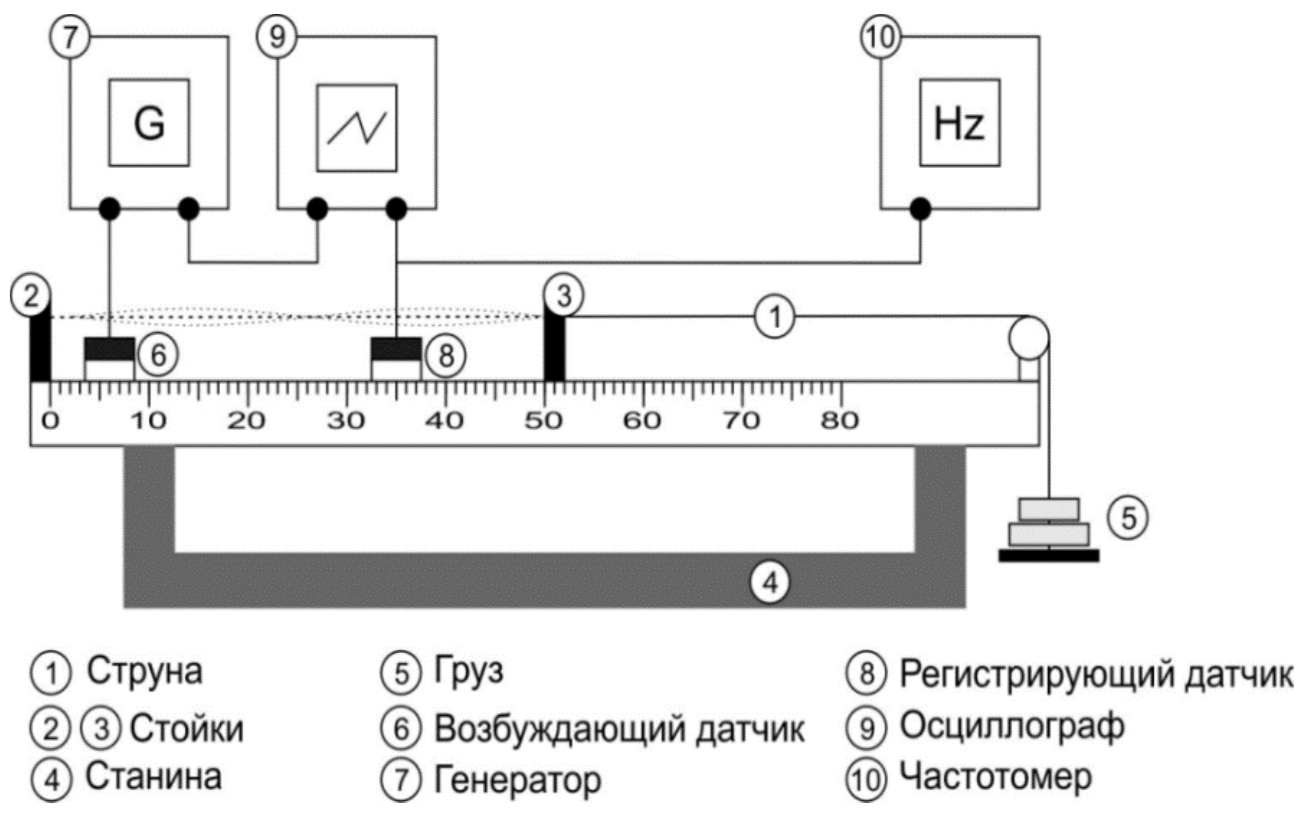
\includegraphics[scale=0.5]{1}
\caption{Экспериментальная установка}
\end{figure}


При возбуждении стоячей волны на экране осциллографа в режиме развертки должен появиться сигнал синусоидально формы. При чрезмерном возбуждении вид синусоиды искажается, что свидетельствует об отклонении от линейного режима. В двухканальном режиме осциллографа можно сравнить опорный (подаваемый одновременно на возбудитель колебаний 6 и канал CH1 осциллографа) и основной (снимаемый с датчика 8) сигналы — в отсутствие нелинейных искажений они должны совпадать. Кроме того, в режиме сложения сигналов (X–Y) на экране должен прорисовываться эллипс правильной формы.

Дополнительным критерием того, что частота гармоники определена верно, является симметричность «резонансной кривой» — амплитудно-частотной характеристики системы (Рис. 5). А именно, при подходе к резонансной частоте со стороны как высоких, так и со стороны низких частот, макси-мум сигнала наблюдается при одном и том же значении частоты.

\section{Ход работы}
\subsection{Визуальное наблюдение стоячих волн}
\begin{itemize}

\item Освободите зажим струны на стойке 3, установить длину струны $L = 50\text{см}$. Натяните струну, поставив на платформу грузы ( $F \approx 1$ кг) (учтите вес платформы и крепежа). Осторожно зажмите струну в стойке, не деформируя струну. Возбуждающий датчик 6 должен располагаться рядом с неподвижной стойкой 2, т.е. вблизи узла стоячей волны.

\item Проведите предварительные расчёты. Оцените скорость распространения волн по формуле (2), используя табличное значение плотности стали ($\rho_\text{ст} = 7,8 \frac{\text{г}}{\text{см}^3}$) и приняв диаметр струны равным $d \approx 0,3$ мм. Для заданных значений длины струны и силы натяжения рассчитайте частоту основной гармоники $\nu_1$ согласно (9).
\[u = \sqrt{\frac{T}{\rho_l}} \approx 67,3 \frac{\text{м}}{\text{c}}\]
\[\nu_n = \frac{u}{\lambda_n}=\frac{n}{2L}\sqrt{\frac{T}{\rho_l}}\]
\item Включите в сеть звуковой генератор и частотомер. Установите на генераторе тип сигнала — синусоидальный, частоту основной гармоники $\nu_1$ и максимальную амплитуду напряжения. При этом сигнал с выхода генератора должен быть подан на возбуждающий датчик 6 (проверьте правильность со-единения проводов!).

\item Медленно меняя частоту звукового генератора в диапазоне $\nu = \nu_1 \pm 5$Гц, добейтесь возбуждения стоячей волны на основной гармонике (одна пучность). Если при колебаниях струна касается регистрирующего датчика 8, осторожно сдвиньте датчик по скамье в сторону подвижного зажима струны 3. Определите частоту первой гармоники по частотомеру.

\item Увеличив частоту в 2 раза, получите картину стоячих волн на второй гармонике, а затем и на более высоких гармониках. Обычно визуально удается наблюдать до 5-7 гармоник. Запишите значения частот стоячих волн, которые удастся пронаблюдать.
\end{itemize}
\subsection{Регистрация стоячих волн с помощью осциллографа}
\begin{itemize}


\item	Визуально настройте струну на основной гармонике, не меняя нагрузку струны и её длину. Установите регистрирующий датчик 8 в центре под струной (в пучности стоячей волны). Уменьшите уровень выходного сигнала генератора так, чтобы при колебаниях струна не касалась датчика. Проверьте правильность соединения проводов. Сигнал колебаний струны с регистрирующего датчика 8 (основной сигнал) подается на вход канала CH2(Y) осциллографа. На вход канала CH1(X) подается опорный сигнал с генератора на частоте возбуждения струны.

\item	Включите осциллограф в сеть и проверьте его настройку. Для наблюдения колебаний струны в одноканальном режиме переключатель режима работы MODE блока вертикального отклонения должен стоять в положении CH2; тумблер режима работы канала Y — в положение AC; на блоке синхронизации установите SOURCE — CH2. Установите такие значения коэффициента усиления канала Y (VOLTS/DIV); постоянную времени развертки (TIME/DIV) и уровень синхронизации (LEVEL), чтобы на экране было удобно наблюдать форму сигнала.

Подстройте частоту $\nu$ генератора так, чтобы амплитуда сигнала была максимальна. Добейтесь отсутствия нелинейных искажений, уменьшая уровень возбуждения (амплитуду напряжения генератора) и подстраивая при этом частоту так, чтобы она соответствовала максимуму сигнала. Запишите окончательное значение частоты основной гармоники $\nu_1$.

\item Проведите измерение частот не менее 5 нечетных ( $n= 1, 3, 5, 7, 9$) гармоник стоячих волн при длине струны 50 см и массе грузов $\approx$1 кг. Для наблюдения нечетных гармоник регистрирующий датчик следует размещать в центре под струной (как для основной гармоники).

\item Измерьте частоты четных ($n= 2, 4, …$) гармоник. Для этого осторожно смещайте регистрирующий датчик 8 по станине в предварительно рассчитанные положения пучностей. Во избежание взаимного влияния («резонирования») датчиков регистрирующий датчик следует сдвигать в строну подвижного зажима струны 3.

\item Проведите опыты пп. 8 и 9 не менее, чем для пяти различных натяжений струны. При изменении нагрузки следует ослабить зажим струны в стойке 3, положить груз на чашку и вновь осторожно зажать струну.

Максимальная нагрузка — не выше 3,5 кг!

\item Благодаря высокой добротности струны, возможно возбуждение её колебаний при кратных частотах генератора, меньших , чем $\nu_1$. Для наблюде-ния явления переключите осциллограф в режим (X-Y) и настройте установку на наблюдение основной гармоники. Затем уменьшите частоту возбуждения в	два раза, установив на генераторе $\nu = \nu_1/2$. На экране осциллографа должна наблюдаться фигура Лиссажу с одним самопересечением. Зарисуйте (или сфотографируйте) наблюдаемую фигуру. Постарайтесь объяснить явление.

\item Определите добротность $Q$ струны как колебательной системы, измерив её амплитудно-частотную характеристику (АЧХ) вблизи одной из резонансных частот (в качестве таковых рекомендуется выбрать 1 или 3) для нескольких натяжений струны (по указанию преподавателя).

Для расчётов воспользуйтесь известным из теории колебаний результатом: добротность колебательной системы связана с резонансной частотой $\nu_\text{рез}$ и шириной резонансной кривой $\Delta \nu$    соотношением
\[Q = \frac{\nu_\text{рез}}{\Delta \nu}\]
где ширина резонансной кривой $\Delta \nu$ измеряется на уровне амплитуды, состовляющей 0,7 от амплитуды в резонансе (Рис. 3)
\begin{figure}[h]
\centering
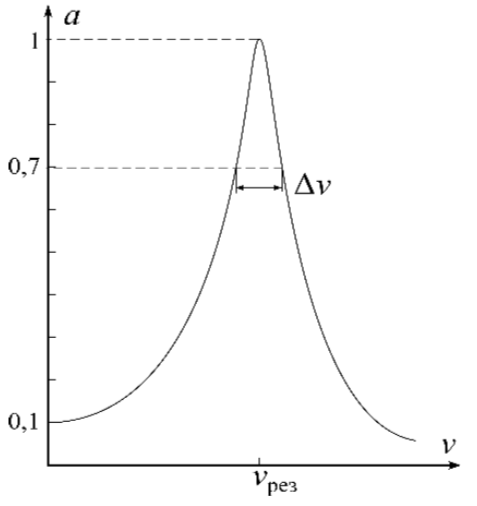
\includegraphics[scale=0.5]{3}
\caption{AЧХ вынужденных колебаний (линенйный режим возбуждения)}
\end{figure}


\end{itemize}
\section{Измерение и обработка дынных}
\begin{table}[h]
\centering
\begin{tabular}{|c|p{1.5cm}|p{1.5cm}|p{1.5cm}|p{1.5cm}|p{1.5cm}|p{1.5cm}|}

\hline
$\text{№}$ & 1 & 2 & 3 & 4 & 5 & 6\\ \hline
$m$ & & & & & & \\ \hline
\end{tabular}
\caption{измерение массы грузиков}
\end{table}

\begin{table}[h]
\centering
\begin{tabular}{|p{1cm}|p{1cm}|p{1cm}|p{1cm}|p{1cm}|p{1cm}|p{1cm}|}

\hline
$n$ & 1 & 2 & 3 & 4 & 5 & 6\\ \hline
$f$, Гц & & & & & &\\ \hline
$f$, Гц & & & & & &\\ \hline
$f$, Гц & & & & & &\\ \hline
$f$, Гц & & & & & &\\ \hline
$f$, Гц & & & & & &\\ \hline
\end{tabular}
\caption{Измерение частоты для $n$ количества полуволн при натяжении струны $T_1$}
\end{table}
\begin{table}[h]
\centering
\begin{tabular}{|p{1cm}|p{1cm}|p{1cm}|p{1cm}|p{1cm}|p{1cm}|p{1cm}|}

\hline
$n$ & 1 & 2 & 3 & 4 & 5 & 6\\ \hline
$f$, Гц & & & & & &\\ \hline
$f$, Гц & & & & & &\\ \hline
$f$, Гц & & & & & &\\ \hline
$f$, Гц & & & & & &\\ \hline
$f$, Гц & & & & & &\\ \hline
\end{tabular}
\caption{Измерение частоты для $n$ количества полуволн при натяжении струны $T_2$}
\end{table}
\begin{table}[h]
\centering
\begin{tabular}{|p{1cm}|p{1cm}|p{1cm}|p{1cm}|p{1cm}|p{1cm}|p{1cm}|}

\hline
$n$ & 1 & 2 & 3 & 4 & 5 & 6\\ \hline
$f$, Гц & & & & & &\\ \hline
$f$, Гц & & & & & &\\ \hline
$f$, Гц & & & & & &\\ \hline
$f$, Гц & & & & & &\\ \hline
$f$, Гц & & & & & &\\ \hline
\end{tabular}
\caption{Измерение частоты для $n$ количества полуволн при натяжении струны $T_3$}
\end{table}
\begin{table}[h]
\centering
\begin{tabular}{|p{1cm}|p{1cm}|p{1cm}|p{1cm}|p{1cm}|p{1cm}|p{1cm}|}

\hline
$n$ & 1 & 2 & 3 & 4 & 5 & 6\\ \hline
$f$, Гц & & & & & &\\ \hline
$f$, Гц & & & & & &\\ \hline
$f$, Гц & & & & & &\\ \hline
$f$, Гц & & & & & &\\ \hline
$f$, Гц & & & & & &\\ \hline
\end{tabular}
\caption{Измерение частоты для $n$ количества полуволн при натяжении струны $T_4$}
\end{table}
\begin{table}[h]
\centering
\begin{tabular}{|p{1cm}|p{1cm}|p{1cm}|p{1cm}|p{1cm}|p{1cm}|p{1cm}|}

\hline
$n$ & 1 & 2 & 3 & 4 & 5 & 6\\ \hline
$f$, Гц & & & & & &\\ \hline
$f$, Гц & & & & & &\\ \hline
$f$, Гц & & & & & &\\ \hline
$f$, Гц & & & & & &\\ \hline
$f$, Гц & & & & & &\\ \hline
\end{tabular}
\caption{Измерение частоты для $n$ количества полуволн при натяжении струны $T_5$}
\end{table}
\begin{table}[h]
\centering
\begin{tabular}{|p{1cm}|p{1cm}|p{1cm}|p{1cm}|p{1cm}|p{1cm}|p{1cm}|}

\hline
$n$ & 1 & 2 & 3 & 4 & 5 & 6\\ \hline
$f$, Гц & & & & & &\\ \hline
$f$, Гц & & & & & &\\ \hline
$f$, Гц & & & & & &\\ \hline
$f$, Гц & & & & & &\\ \hline
$f$, Гц & & & & & &\\ \hline
\end{tabular}
\caption{Измерение частоты для $n$ количества полуволн при натяжении струны $T_6$}
\end{table}
\end{document}